\documentclass[../thesis.tex]{subfiles}
\begin{document}

\chapter{theory}
\label{chp:theory}


\section{governing equations}

When deriving the equations necessary to model the fluid flow, conservation laws have to be applied to each fluid element. The balances looked at are:
\begin{enumerate}
	\item conservation of mass
	\item conservation of momentum
\end{enumerate}
Each of these balances can be created for a small volume element. This element must meet the condition that it's macroscopic properties such as velocity, pressure, temperature or density can be sufficiently described by the average value within the fluid element \cite{versteeg2007introduction}. To explain the set of equations the fluid element is modelled as a cuboid as shown in \autoref{fig:fluidelement}.

\begin{figure}[htbp]
	\centering
	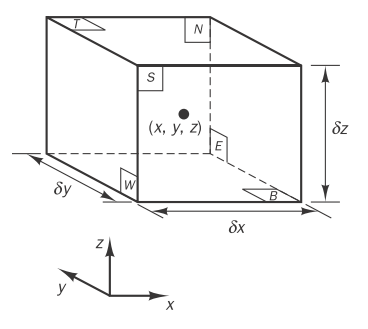
\includegraphics[scale=0.5]{Fluidelement}
	\caption{fluid element}
	\label{fig:fluidelement}
\end{figure}

As shown the cuboid has six faces. The face labelled $ N $ is called North, $ S $ is called South, $ W $ is called West and $ E $ is called East. The top and bottom faces are called $ B $ for Bottom and $ T $ for Top. The cells centre is located at the coordinates ($ x,y,z $). All properties mentioned above are space and time dependant. For simplicity and readability the dependency of space and time is not written within the equations so that for example the temperature for the location ($ x,y,z $) at the time $ t $ is written as:

\begin{equation}
	T(x,y,z,t) = T
\end{equation}

An equal treatment is done for the derivatives. The derivative regarding the coordinate $ x $ for the variable $ T $ is written like this:

\begin{equation}
	\dfrac{\partial T(x,y,z,t)}{\partial x} = \dfrac{\partial T}{\partial x}
\end{equation}

All values calculated are values for the cell's centre. To obtain a value at a cell's face interpolation is needed. As good initial guess the first to terms of a taylor series expansion are used. In the example of the density $ \rho$ at the West face the equation to calculated the value looks like this:

\begin{equation}
	\rho_{\mathrm{West}} = \rho -  \dfrac{\partial \rho}{\partial x} \cdot \dfrac{1}{2} \cdot \delta x
\end{equation}

\subsection{mass conservation}

The first balance looked at is the mass conservation. For each fluid element the rate of increase can be written as:

\begin{equation}
	\label{eq:FE_mb}
	\dfrac{\partial m}{\partial t} = \dfrac{\partial}{\partial t}(\rho \cdot \delta x \cdot \delta y \cdot \delta z) = \dfrac{\partial \rho}{\partial t} \cdot V + S
\end{equation}

The term $ \frac{\partial m}{\partial t} $ describes the changing mass within the fluid element. $ \frac{\partial \rho}{\partial t} \cdot V $ describes the flow across the boundary faces and $ S $ is a source term. For simplicity the source term is dropped from \autoref{eq:FE_mb} so it can be simplified to:

\begin{equation}
	\dfrac{\partial}{\partial t}(\rho \cdot \delta x \cdot \delta y \cdot \delta z) = \dfrac{\partial \rho}{\partial t} \cdot \delta x \cdot \delta y \cdot \delta z
\end{equation}

The mass flow across the boundary faces $ i $ can be written as:

\begin{equation}
	m_i = \rho \cdot u_i \cdot A_i
\end{equation}

The term $ u_i $ represents the velocity normal to the face $ A_i$ and $ \rho $ is the density. The velocity in $x$ direction is named $u$, the velocity in $y$ direction is named $w$ and the velocity in $z$ direction is named $w$. With that the mass balance for the hole cuboid can be written as:

\begin{eqnarray}
	\label{eq:FE_mb_large}
	\dfrac{\partial}{\partial t} \cdot (\rho \delta x \delta y \delta z) & = & \left[ \rho u -  \dfrac{\partial \rho u}{\partial x} \cdot \dfrac{1}{2} \cdot \delta x \right] \delta y \delta z -
	\left[ \rho u +  \dfrac{\partial \rho u}{\partial x} \cdot \dfrac{1}{2} \cdot \delta x \right] \delta y \delta z \nonumber \\
	& & + \left[ \rho v -  \dfrac{\partial \rho v}{\partial y} \cdot \dfrac{1}{2} \cdot \delta y \right] \delta x \delta z -
	\left[ \rho v +  \dfrac{\partial \rho v}{\partial y} \cdot \dfrac{1}{2} \cdot \delta y \right] \delta x \delta z \\
	& & + \left[ \rho w -  \dfrac{\partial \rho w}{\partial z} \cdot \dfrac{1}{2} \cdot \delta z \right] \delta x\delta y -
	\left[ \rho w +  \dfrac{\partial \rho w}{\partial z} \cdot \dfrac{1}{2} \cdot \delta z \right] \delta x \delta y \nonumber
\end{eqnarray}

Each contribution to the mass flow is shown in \autoref{fig:fluidelement_massflow}.

\begin{figure}[htbp]
	\centering
	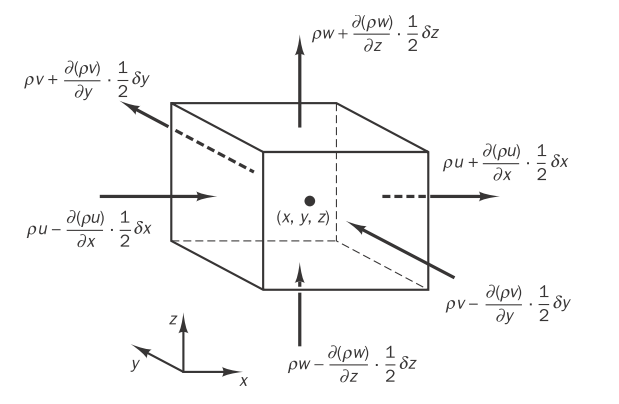
\includegraphics[scale=0.6]{Fluidelement_flow}
	\caption{fluid element mass flow}
	\label{fig:fluidelement_massflow}
\end{figure}

\autoref{eq:FE_mb_large} can be simplified to:

\begin{equation}
	\dfrac{\partial \rho}{\partial t} \cdot (\delta x \delta y \delta z) = - \dfrac{\partial \rho u}{\partial x} \cdot \delta x \delta y \delta z - \dfrac{\partial \rho v}{\partial y} \cdot \delta y \delta x \delta z - \dfrac{\partial \rho w}{\partial z} \cdot \delta z \delta x \delta y
\end{equation}

\begin{equation}
	\label{eq:FE_mb_short}
	\dfrac{\partial \rho}{\partial t} + \dfrac{\partial \rho u}{\partial x} + \dfrac{\partial \rho v}{\partial y} + \dfrac{\partial \rho w}{\partial z} = 0
\end{equation}

For an incompressible fluid \autoref{eq:FE_mb_short} can be further shortened because the density $ \rho $ does not change over time.

\begin{equation}
	\mathrm{div}(\textbf{u}) = 0
\end{equation}

\subsection{momentum conservation}
\label{sec:moment_conv}

When looking at the rate of momentum change of a fluid element the sum of all forces on the fluid particle has to be taken into account due to Newton's second law \cite{versteeg2007introduction}. Two different type of forces working on a fluid particle can be distinguished. On one hand there are surface forces which contain pressure forces, viscous forces and gravity force. On the other hand there are body forces which contain centrifugal forces, Coriolis force, and electromagnetic force. Both type of forces will be presented by different terms within the momentum equation.

When looking at a cuboid fluid element nine different viscous stresses $ \tau_{ij} $ can be found as shown in \autoref{fig:fluidelement_stress}. The index $ i $ indicates the face the viscous stress is working on, because it is the normal vector's direction on that face. The index $ j $ indicates the direction of the stress. 

\begin{figure}[htbp]
	\centering
	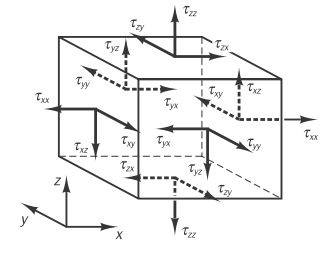
\includegraphics[scale=0.7]{Fluidelement_stress}
	\caption{fluid element stress components}
	\label{fig:fluidelement_stress}
\end{figure}

Looking at the forces in x-direction the stress components $ \tau_{xx}$ , $ \tau_{yx}$, $ \tau_{zx}$ as well as the pressure $ p $ need to be taken into account. All terms including their location can be found in \autoref{fig:fluidelement_x_stress}. The terms e.g. $p - \frac{\partial p}{\partial x} \cdot \frac{1}{2} \cdot \delta x$ result from the assumption that the value on the surface can described by the first two terms of a Taylor series expansion.

\begin{figure}[htbp]
	\centering
	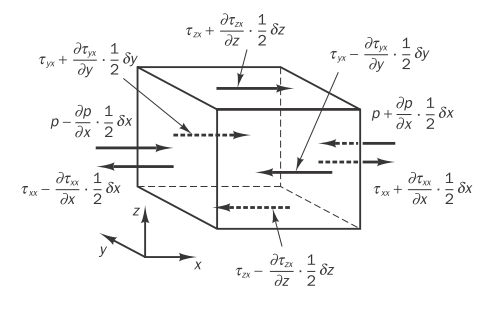
\includegraphics[scale=0.7]{Fluidelement_x_stress}
	\caption{fluid element stress in x direction}
	\label{fig:fluidelement_x_stress}
\end{figure}

The sum of all forces on the East and West face can written as:

\begin{equation}
	\begin{split}
		& \left[ 
		\left( p - \dfrac{\partial p}{\partial x} \dfrac{1}{2} \delta x \right) - 
		\left( \tau_{xx} - \dfrac{\partial \tau_{xx}}{\partial x} \dfrac{1}{2} \delta x \right)
		\right] \delta y \delta z \\ & + 
		\left[ - 
		\left( p + \dfrac{\partial p}{\partial x} \dfrac{1}{2} \delta x \right) - 
		\left( \tau_{xx} + \dfrac{\partial \tau_{xx}}{\partial x} \dfrac{1}{2} \delta x \right)
		\right] \delta y \delta z \\ & =
		\left( - \dfrac{\partial p}{\partial x} + \dfrac{\partial \tau_{xx}}{\partial x} \right) \delta x \delta y \delta z
	\end{split}
\end{equation}

Doing the same for the remaining faces results for the combination of the north and south faces in:

\begin{equation}
	- \left( \tau_{yx} + \dfrac{\partial \tau_{yx}}{\partial y} \dfrac{1}{2} \delta y \right) \delta x \delta z + 
	\left( \tau_{yx} + \dfrac{\partial \tau_{yx}}{\partial y} \dfrac{1}{2} \delta y \right) \delta x \delta z = 
	\dfrac{\partial \tau_{yx}}{\partial y} \delta x \delta y \delta z
\end{equation}

and for the combination of top and bottom face:

\begin{equation}
	- \left( \tau_{zx} + \dfrac{\partial \tau_{zx}}{\partial z} \dfrac{1}{2} \delta z \right) \delta x \delta y + 
	\left( \tau_{zx} + \dfrac{\partial \tau_{zx}}{\partial z} \dfrac{1}{2} \delta z \right) \delta x \delta y = 
	\dfrac{\partial \tau_{zx}}{\partial y} \delta x \delta y \delta z
\end{equation}

The resulting surface force per unit volume ($\delta x \delta y \delta z$) in x-direction $ F_x $ is equal to:

\begin{equation}
	F_x = \dfrac{\partial (- p + \tau_{xx})}{\partial x} + \dfrac{\tau_{yx}}{\partial y} + \dfrac{\partial \tau_{zx}}{\partial z}
\end{equation}

With the same approach the forces per unit volume in $ y $ and $ z $ direction can be derived to the form shown in \autoref{eq:sum_Fy} and \autoref{eq:sum_Fz}.

\begin{equation}
	\label{eq:sum_Fy}
	F_y =  \dfrac{\tau_{xy}}{\partial x} + \dfrac{\partial (- p + \tau_{yy})}{\partial y} + \dfrac{\partial \tau_{zy}}{\partial z}
\end{equation}

\begin{equation}
	\label{eq:sum_Fz}
	F_z = \dfrac{\tau_{xz}}{\partial x} + \dfrac{\partial \tau_{yz}}{\partial y} + \dfrac{\partial (- p + \tau_{zz})}{\partial z}
\end{equation}

The resulting momentum equations are:

\begin{eqnarray}
	\rho \dfrac{Du}{Dt} = & \dfrac{\partial (-p + \tau_{xx})}{\partial x} + \dfrac{\tau_{yx}}{\partial y} + \dfrac{\partial \tau_{zx}}{\partial z} + S_{M_x} \\
	\rho \dfrac{Dv}{Dt} = & \dfrac{\tau_{xy}}{\partial x} + \dfrac{\partial (-p + \tau_{yy})}{\partial y} + \dfrac{\partial \tau_{zy}}{\partial z} +  S_{M_y} \\
	\rho \dfrac{Dw}{Dt} = & \dfrac{\tau_{xz}}{\partial x} + \dfrac{\partial \tau_{yz}}{\partial y} + \dfrac{\partial (-p + \tau_{zz})}{\partial z} +
	S_{M_z}
\end{eqnarray}

The terms $S_{M_x}, S_{M_y}, S_{M_z}$ are source terms which represent the body forces. In case of gravity the source term in $z$ direction would be equal to $ -\rho g$.

\section{Navier-Stokes equations}

Within the momentum equations there are the viscous stress components $ \tau_{ij}$. For these unknown variables a calculation method is needed. In most fluids the viscous stress is directly linked to the rate of local deformation $ s $. There are nine different local deformation components, from which six are independent for isotropic fluids. These nine components can be seen in \autoref{fig:fluidelement_stress}, because they occur in the same direction as the viscous stresses. The six independent components can be divided into three elongating deformations $ s_{ii} $, as shown in Equations \ref{eq:stress_x_elong} to \ref{eq:stress_z_elong}, and six shearing linear deformations $ s_{iy} $, shown in Equations \ref{eq:stress_xy_lin} to \ref{eq:stress_yz_lin}. The indexing convention is the same as in \autoref{sec:moment_conv}.

\begin{eqnarray}
	s_{xx} = & \dfrac{\partial u}{\partial x} \label{eq:stress_x_elong} \\[6pt]
	s_{yy} = & \dfrac{\partial v}{\partial y} \label{eq:stress_y_elong}  \\[6pt] 
	s_{zz} = & \dfrac{\partial w}{\partial z} \label{eq:stress_z_elong}
\end{eqnarray}

\begin{eqnarray}
	s_{xy} = & s_{yx} = & \dfrac{1}{2} \cdot \left( \dfrac{\partial u}{\partial y} + \dfrac{\partial v}{\partial x} \right) \label{eq:stress_xy_lin} \\[6pt] 
	s_{xz} = & s_{zx} = & \dfrac{1}{2} \cdot \left( \dfrac{\partial u}{\partial z} + \dfrac{\partial w}{\partial x} \right) \label{eq:stress_xz_lin} \\[6pt] 
	s_{yz} = & s_{zy} = & \dfrac{1}{2} \cdot \left( \dfrac{\partial v}{\partial z} + \dfrac{\partial w}{\partial y} \right)	\label{eq:stress_yz_lin}
\end{eqnarray}

For a Newtonian fluid the viscous stresses are proportional to the local deformation rates.



\section{finite volume method}

To model  fluid flow two concepts have been established. On one side there is the Euler description which looks at a fixed location in space and monitors the changes happening to that given location. On the other side there is the Lagrang description where the model describes the influence on a fluid element following the flow. Both methods are equal so it is possible to convert them into each other. The main focus will be on the Euler description because it is the method used in this work.

In general the finite volume method splits the model into sections that describe the models properties in that region. The number and shape of these sections depend on the given problem and geometry. This mesh has to be initially created by the user.    

\end{document}